\chapter{トポロジー導関数の導出}
\begin{figure}[ht]
	\begin{center}
		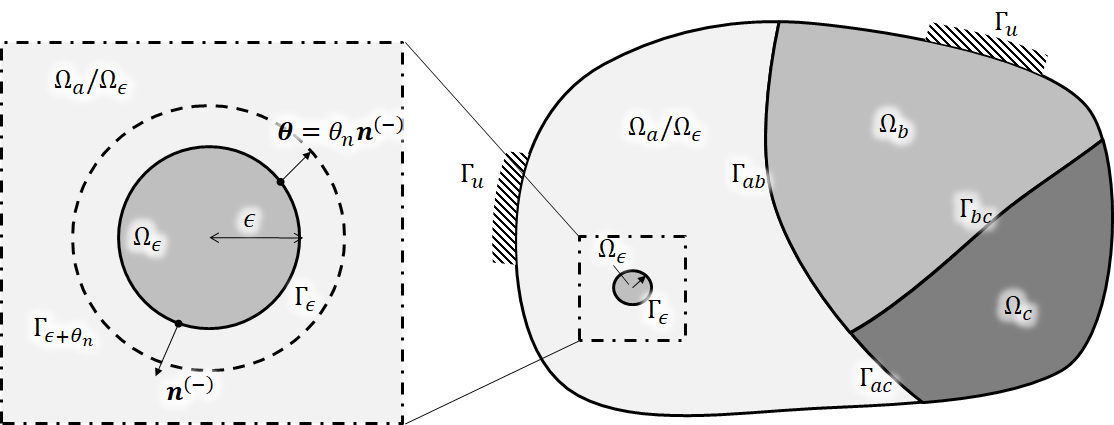
\includegraphics[width=13cm]{./figures/SDforTD.png}
		\caption{Shape derivative for computing the topological derivative}
		\label{fig:TD}
	\end{center}
\end{figure}

$\bm{\theta}$を次式のように設定する.
\begin{align}
	\bm{\theta}=&\theta_{n}\bm{n}^{(-)}	\hspace{1cm}\text{on}\hspace{0.3cm}\Gamma_{\epsilon}\\
	\bm{\theta}=&\bm{0}					\hspace{1.8cm}\text{on}\hspace{0.3cm}\Gamma/\Gamma_{\epsilon}
\end{align}
この時,固有値$\lambda$の形状微分は,\eqref{eq:shape_lambda}に
$\bm{u}=\bm{u}^{\epsilon},\lambda=\lambda^{\epsilon}$を代入することで以下のようになる.
\begin{align}
	&\hspace{0.5cm}D\lambda^{a\rightarrow b}(\Omega_{p\{1\leq p\leq n\}})\cdot\bm{\theta}
	\nonumber
	\\
	=&\int_{\Gamma_\epsilon}(\theta_{n}n_{\gamma}^{(-)}n_{\gamma}^{(-)})
	\Bigr(u_{i,j}^{\epsilon(-)}C_{ijkl}^{b}u_{k,l}^{\epsilon(-)}
	-\lambda^{\epsilon}\rho^{b}u_{i}^{\epsilon(-)}u_{i}^{\epsilon(-)}\Bigl) d\Omega
	\nonumber
	\\
	&+\int_{\Gamma_\epsilon}(\theta_{n}n_{\gamma}^{(-)}n_{\gamma}^{(+)})
	\Bigr(u_{i,j}^{\epsilon(+)}C_{ijkl}^{a}u_{k,l}^{\epsilon(+)}
	-\lambda^{\epsilon}\rho^{a}u_{i}^{\epsilon(+)}u_{i}^{\epsilon(+)}\Bigl) d\Omega
	\nonumber
	\\
	&-\int_{\Gamma_{\epsilon}}(\theta_{n}n_{\gamma}^{(-)}n_{\gamma}^{(-)})
	\Bigr(C_{ijkl}^{b}u_{k,l}^{\epsilon(-)}n_{j}^{(-)}
	-C_{ijkl}^{a}u_{k,l}^{\epsilon(+)}n_{j}^{(+)}\Bigl)
	(u_{i,m}^{\epsilon(-)}n_{m}^{(-)}-u_{i,m}^{\epsilon(+)}n_{m}^{(-)}) d\Gamma
	\nonumber
	\\
	=&\theta_{n}\int_{\Gamma_\epsilon}
	\Bigr(u_{i,j}^{\epsilon(-)}C_{ijkl}^{b}u_{k,l}^{\epsilon(-)}
	-\lambda^{\epsilon}\rho^{b}u_{i}^{\epsilon(-)}u_{i}^{\epsilon(-)}\Bigl) d\Omega
	\nonumber
	\\
	&-\theta_{n}\int_{\Gamma_\epsilon}
	\Bigr(u_{i,j}^{\epsilon(+)}C_{ijkl}^{a}u_{k,l}^{\epsilon(+)}
	-\lambda^{\epsilon}\rho^{a}u_{i}^{\epsilon(+)}u_{i}^{\epsilon(+)}\Bigl) d\Omega
	\nonumber
	\\
	&-\theta_{n}\int_{\Gamma_{\epsilon}}
	\Bigr(C_{ijkl}^{b}u_{k,l}^{\epsilon(-)}n_{j}^{(-)}
	+C_{ijkl}^{a}u_{k,l}^{\epsilon(+)}n_{j}^{(-)}\Bigl)
	(u_{i,m}^{\epsilon(-)}n_{m}^{(-)}-u_{i,m}^{\epsilon(+)}n_{m}^{(-)}) d\Gamma
	\label{eq:SDForTD}
	\\
	=&\theta_{n}\int_{\Gamma_\epsilon}
	\Bigr(e^{\epsilon(-)}:\sigma^{\epsilon(-)}
	-\lambda^{\epsilon}\rho^{b}|\bm{u}^{\epsilon(-)}|^{2}\Bigl) d\Omega
	-\theta_{n}\int_{\Gamma_\epsilon}
		\Bigr(e^{\epsilon(+)}:\sigma^{\epsilon(+)}
		-\lambda^{\epsilon}\rho^{a}|\bm{u}^{\epsilon(+)}|^{2}\Bigl) d\Omega
	\nonumber
	\\
	&-\theta_{n}\int_{\Gamma_{\epsilon}}\Bigl\{
	\Bigr(t_{i}^{\epsilon(-)}+t_{i}^{\epsilon(+)}\Bigl)
		\Bigl(\frac{\partial u_{i}^{\epsilon(-)}}{\partial n}-\frac{\partial u_{i}^{\epsilon(+)}}{\partial n}\Bigr)
	\Bigl\}d\Gamma
	\label{eq:SDForTDRTh}
\end{align}

\begin{figure}[ht]
	\begin{center}
		\includegraphics[height=5cm]{./figures/Rth.png}
		\caption{$(R,\theta)$ coordinate}
		\label{fig:Rth}
	\end{center}
\end{figure}
ここで,
\begin{align}
	x_{1}-z_{1}=R\cos(\theta)
	\nonumber
	\\
	x_{2}-z_{2}=R\sin(\theta)
	\label{eq:xyToRTh}
\end{align}
と座標変換すると$R,\theta$方向の変位は以下のようになる.
\begin{align}
	u_{R}^{\epsilon(-)}(r,\theta)=&\hat{w}_{r}^{(I-)}(\theta)
	+\epsilon\hat{w}_{r}^{(I\hspace{-.15em}I-)}(r,\theta)+O(\epsilon^2)
	\nonumber
	\\
	u_{\theta}^{\epsilon(-)}(r,\theta)=&\hat{w}_{\theta}^{(I-)}(\theta)
	+\epsilon\hat{w}_{\theta}^{(I\hspace{-.15em}I-)}(r,\theta)+O(\epsilon^2)
	\nonumber
	\\
	u_{R}^{\epsilon(+)}(R,r,\theta)=&u_{x_{1}}(\bm{x})\cos(\theta)+u_{x_{2}}(\bm{x})\sin(\theta)
	+\epsilon\hat{w}_{r}^{(I\hspace{-.15em}I+)}(r,\theta)+O(\epsilon^2)
	\nonumber
	\\
	u_{\theta}^{\epsilon(+)}(R,r,\theta)=&-u_{x_{1}}(\bm{x})\sin(\theta)+u_{x_{2}}(\bm{x})\cos(\theta)
	+\epsilon\hat{w}_{\theta}^{(I\hspace{-.15em}I+)}(r,\theta)+O(\epsilon^2)
	\label{eq:SDForTD}
\end{align}
$R=\epsilon r$の関係から,
\begin{align}
	\frac{\partial}{\partial R}=\frac{1}{\epsilon}\frac{\partial}{\partial r}
	\label{eq:RTor}
\end{align}
であることに注意して歪みや応力を計算すると以下のようになる.
\begin{align}
	e_{RR}^{\epsilon(-)}-e_{RR}^{\epsilon(+)}
		=&\frac{\partial u_{R}^{\epsilon(-)}}{\partial n}-\frac{\partial u_{R}^{\epsilon(+)}}{\partial n}
		\nonumber
		\\
		=&2A\bigl\{u_{x_{1},x_{1}}(\bm{z})+u_{x_{2},x_{2}}(\bm{z})\bigr\}
		\nonumber
		\\
		&+(\kappa^{a}-1)B\bigl\{u_{x_{1},x_{1}}(\bm{z})-u_{x_{2},x_{2}}(\bm{z})\bigr\}\cos(2\theta)
		\nonumber
		\\
		&+(\kappa^{a}-1)B\bigl\{u_{x_{1},x_{2}}(\bm{z})+u_{x_{2},x_{1}}(\bm{z})\bigr\}\sin(2\theta)+O(\epsilon)
		\nonumber
		\\
	2\Bigl\{e_{R\theta}^{\epsilon(-)}-e_{R\theta}^{\epsilon(+)}\Bigr\}
		=&\frac{\partial u_{\theta}^{\epsilon(-)}}{\partial n}-\frac{\partial u_{\theta}^{\epsilon(+)}}{\partial n}
		\nonumber
		\\
		=&-\bigl\{u_{x_{1},x_{1}}(\bm{z})-u_{x_{2},x_{2}}(\bm{z})\bigr\}
		\nonumber
		\\
		&-(\kappa^{a}+1)B\bigl\{u_{x_{1},x_{1}}(\bm{z})-u_{x_{2},x_{2}}(\bm{z})\bigr\}\cos(2\theta)
		\nonumber
		\\
		&+(\kappa^{a}+1)B\bigl\{u_{x_{1},x_{2}}(\bm{z})+u_{x_{2},x_{1}}(\bm{z})\bigr\}\sin(2\theta)+O(\epsilon)
		\nonumber
		\\
	e_{\theta\theta}^{\epsilon(-)}=e_{\theta\theta}^{\epsilon(+)}
		=&\frac{(\kappa^{b}-1)}{2}C\bigl\{u_{x_{1},x_{1}}(\bm{z})+u_{x_{2},x_{2}}(\bm{z})\bigr\}
		\nonumber
		\\
		&-\frac{D}{2}\bigl\{u_{x_{1},x_{1}}(\bm{z})-u_{x_{2},x_{2}}(\bm{z})\bigr\}\cos(2\theta)
		\nonumber
		\\
		&-\frac{D}{2}\bigl\{u_{x_{1},x_{2}}(\bm{z})+u_{x_{2},x_{1}}(\bm{z})\bigr\}\sin(2\theta)+O(\epsilon)
		\nonumber
		\\
	\sigma_{RR}^{\epsilon(-)}=\sigma_{RR}^{\epsilon(+)}
		=&2\mu^{b}C\bigl\{u_{x_{1},x_{1}}(\bm{z})+u_{x_{2},x_{2}}(\bm{z})\bigr\}
		\nonumber
		\\
		&+\mu^{b}D\bigl\{u_{x_{1},x_{1}}(\bm{z})-u_{x_{2},x_{2}}(\bm{z})\bigr\}\cos(2\theta)
		\nonumber
		\\
		&+\mu^{b}D\bigl\{u_{x_{1},x_{2}}(\bm{z})+u_{x_{2},x_{1}}(\bm{z})\bigr\}\sin(2\theta)+O(\epsilon)
		\nonumber
		\\
	\sigma_{R\theta}^{\epsilon(-)}=\sigma_{R\theta}^{\epsilon(+)}
		=&-\mu^{b}D\bigl\{u_{x_{1},x_{1}}(\bm{z})-u_{x_{2},x_{2}}(\bm{z})\bigr\}\cos(2\theta)
		\nonumber
		\\
		&+\mu^{b}D\bigl\{u_{x_{1},x_{2}}(\bm{z})+u_{x_{2},x_{1}}(\bm{z})\bigr\}\sin(2\theta)+O(\epsilon)
		\nonumber
		\\
	\sigma_{\theta\theta}^{\epsilon(-)}-\sigma_{\theta\theta}^{\epsilon(+)}
		=&-4\mu^{a}A\bigl\{u_{x_{1},x_{1}}(\bm{z})+u_{x_{2},x_{2}}(\bm{z})\bigr\}
		\nonumber
		\\
		&+4\mu^{a}B\bigl\{u_{x_{1},x_{1}}(\bm{z})-u_{x_{2},x_{2}}(\bm{z})\bigr\}\cos(2\theta)
		\nonumber
		\\
		&+4\mu^{a}B\bigl\{u_{x_{1},x_{2}}(\bm{z})+u_{x_{2},x_{1}}(\bm{z})\bigr\}\sin(2\theta)+O(\epsilon)
	\label{eq:eThThOutEpsSol}
\end{align}
ただし,
\begin{align}
	A=&\frac{\mu^{a}(\kappa^{b}-1)-\mu^{b}(\kappa^{a}-1)}
	{\bigl(\mu^{a}(\kappa^{b}-1)+2\mu^{b}\bigr)(\kappa^{a}-1)}
	\nonumber
	\\
	B=&\frac{\mu^{a}-\mu^{b}}
	{\mu^{a}+\kappa^{a}\mu^{b}}
	\nonumber
	\\
	C=&\frac{\mu^{a}(\kappa^{a}+1)}
	{\bigl(\mu^{a}(\kappa^{b}-1)+2\mu^{b}\bigr)(\kappa^{a}-1)}
	\nonumber
	\\
	D=&\frac{\mu^{a}(\kappa^{a}+1)}
	{\mu^{a}+\kappa^{a}\mu^{b}}
	\label{eq:eThThOutEpsSol}
\end{align}
とおいた.式\eqref{eq:SDForTDRTh}と$\lambda^\epsilon=\lambda+O(\epsilon)$を式\eqref{eq:eThThOutEpsSol}に代入すると,形状微分は以下のようになる
\begin{align}
	&D\lambda^{a\rightarrow b}(\Omega_{p\{1\leq p\leq n\}})\cdot\bm{\theta}
	\nonumber
	\\
	=&\theta_{n}\epsilon\int_{0}^{2\pi}
		\Bigr(\bigl\{e_{RR}^{\epsilon(-)}-e_{RR}^{\epsilon(+)}\bigr\}\sigma_{RR}^{\epsilon(-)}
		+2\bigl\{e_{R\theta}^{\epsilon(-)}-e_{R\theta}^{\epsilon(+)}\bigr\}\sigma_{R\theta}^{\epsilon(-)}
		+e_{\theta\theta}^{\epsilon(-)}\bigl\{\sigma_{\theta\theta}^{\epsilon(-)}-\sigma_{\theta\theta}^{\epsilon(+)}\bigr\}
		\Bigl) d\theta
		\nonumber
		\\
	&-\theta_{n}\epsilon\int_{0}^{2\pi}
		\lambda^{\epsilon}\Bigr(
		\rho^{b}|\bm{u}^{\epsilon(-)}|^{2}-\rho^{a}|\bm{u}^{\epsilon(+)}|^{2}
		\Bigl) d\theta
		\nonumber
		\\
	&-\theta_{n}\epsilon\int_{0}^{2\pi}\Bigr(
		2\bigl\{e_{RR}^{\epsilon(-)}-e_{RR}^{\epsilon(+)}\bigr\}\sigma_{RR}^{\epsilon(-)}
		+4\bigl\{e_{R\theta}^{\epsilon(-)}-e_{R\theta}^{\epsilon(+)}\bigr\}\sigma_{R\theta}^{\epsilon(-)}
		\Bigl) d\theta
	\nonumber
	\\
	=&\theta_{n}\epsilon\int_{0}^{2\pi}
		\Bigr(-\bigl\{e_{RR}^{\epsilon(-)}-e_{RR}^{\epsilon(+)}\bigr\}\sigma_{RR}^{\epsilon(-)}
		-2\bigl\{e_{R\theta}^{\epsilon(-)}-e_{R\theta}^{\epsilon(+)}\bigr\}\sigma_{R\theta}^{\epsilon(-)}
		+e_{\theta\theta}^{\epsilon(-)}\bigl\{\sigma_{\theta\theta}^{\epsilon(-)}-\sigma_{\theta\theta}^{\epsilon(+)}\bigr\}
		\Bigl) d\theta
		\nonumber
		\\
	&-\theta_{n}\epsilon\int_{0}^{2\pi}
		\lambda^{\epsilon}\Bigr(
		\rho^{b}|\bm{u}^{\epsilon(-)}|^{2}-\rho^{a}|\bm{u}^{\epsilon(+)}|^{2}
		\Bigl) d\theta
	\nonumber
	\\
	=&2\pi\epsilon\theta_{n}\Bigl[
	-2\bigl\{\mu^{a}(\kappa^{b}-1)+2\mu^{b}\bigr\}AC
		\bigl\{u_{x_{1},x_{1}}(\bm{z})+u_{x_{2},x_{2}}(\bm{z})\bigr\}^2
		\nonumber
		\\
	&\hspace{1cm}-\bigl(\mu^{b}\kappa^{a}+\mu^{a}\bigr)BD
		\bigl\{u_{x_{1},x_{1}}(\bm{z})-u_{x_{2},x_{2}}(\bm{z})\bigr\}^2
		\nonumber
		\\
	&\hspace{1cm}-\bigl(\mu^{b}\kappa^{a}+\mu^{a}\bigr)BD
		\bigl\{u_{x_{1},x_{2}}(\bm{z})+u_{x_{2},x_{1}}(\bm{z})\bigr\}^2
		\nonumber
		\\
	&\hspace{1cm}-\lambda\Bigr(\rho^{b}-\rho^{a}\Bigl)|\bm{u}(\bm{z})|^{2}
	\Bigr]+O(\epsilon^2)
	\nonumber
	\\
	=&2\pi\epsilon\theta_{n}\Bigl[
	-\frac{2\mu^{a}(\kappa^{a}+1)\Bigl\{\mu^{a}(\kappa^{b}-1)-\mu^{b}(\kappa^{a}-1)\Bigl\}}
			{\bigl(\mu^{a}(\kappa^{b}-1)+2\mu^{b}\bigr)(\kappa^{a}-1)^2}
		\bigl\{u_{x_{1},x_{1}}(\bm{z})+u_{x_{2},x_{2}}(\bm{z})\bigr\}^2
		\nonumber
		\\
	&\hspace{1cm}-\frac{\mu^{a}(\mu^{a}-\mu^{b})(\kappa^{a}+1)}{\mu^{a}+\kappa^{a}\mu^{b}}
		\bigl\{u_{x_{1},x_{1}}(\bm{z})-u_{x_{2},x_{2}}(\bm{z})\bigr\}^2
		\nonumber
		\\
	&\hspace{1cm}-\frac{\mu^{a}(\mu^{a}-\mu^{b})(\kappa^{a}+1)}{\mu^{a}+\kappa^{a}\mu^{b}}
		\bigl\{u_{x_{1},x_{2}}(\bm{z})+u_{x_{2},x_{1}}(\bm{z})\bigr\}^2
		\nonumber
		\\
	&\hspace{1cm}-\lambda\Bigr(\rho^{b}-\rho^{a}\Bigl)|\bm{u}(\bm{z})|^{2}
	\Bigr]+O(\epsilon^2)
	\label{eq:SDForTDRTh}
\end{align}
ゆえに,式\eqref{eq:TSSen}より,トポロジー導関数は以下のように導出される.
\begin{align}
	D_{T}\lambda^{a\rightarrow b}=&\lim_{\epsilon \to 0} \frac{D\lambda^{a\rightarrow b}\cdot\bm{\theta}}{2\pi\epsilon\theta_{n}}
	\nonumber
	\\
	=&\frac{2\mu^{a}(\kappa^{a}+1)\Bigl\{\mu^{b}(\kappa^{a}-1)-\mu^{a}(\kappa^{b}-1)\Bigl\}}
			{\bigl(\mu^{a}(\kappa^{b}-1)+2\mu^{b}\bigr)(\kappa^{a}-1)^2}
		\bigl\{u_{x_{1},x_{1}}(\bm{z})+u_{x_{2},x_{2}}(\bm{z})\bigr\}^2
		\nonumber
		\\
	&+\frac{\mu^{a}(\mu^{b}-\mu^{a})(\kappa^{a}+1)}{\mu^{a}+\kappa^{a}\mu^{b}}
		\bigl\{u_{x_{1},x_{1}}(\bm{z})-u_{x_{2},x_{2}}(\bm{z})\bigr\}^2
		\nonumber
		\\
	&+\frac{\mu^{a}(\mu^{b}-\mu^{a})(\kappa^{a}+1)}{\mu^{a}+\kappa^{a}\mu^{b}}
		\bigl\{u_{x_{1},x_{2}}(\bm{z})+u_{x_{2},x_{1}}(\bm{z})\bigr\}^2
		\nonumber
		\\
	&-\lambda\Bigr(\rho^{b}-\rho^{a}\Bigl)|\bm{u}(\bm{z})|^{2}
	\label{eq:TD}
\end{align}
